% ==============================================================================
% TCC - Nome do Aluno
% Capítulo 3 - Especificação de Requisitos
% ==============================================================================
\chapter{Algoritmo A*}
\label{sec-aestrela}

\section{O Algoritmo}
\label{sec-aestrela-algoritmo}
O algoritmo A* (lê-se "A estrela") também conhecido como busca A* é um algoritmo de busca informatizada em grafos. Foi proposta originalmente em (buscar referência) e pode ser visto como uma adaptação do algoritmo de Dijkstra (apresentado no capítulo \ref{sec-dijkstra}) em que, ao invés de se calcular a melhor rota de um ponto de partida para todos os demais vértices do grafo, se estabelece uma boa rota (ou mesmo a rota ótima\footnote{A garantia do valor ótimo do algoritmo depende de fatores que serão discutidos na subseção \ref{sec-aestrela-algoritmo-heuristica}.}) partindo do vértice origem a um vértice destino. Isso é feito realizando "podas" do caminho de forma que não seja necessário visitar todos os vértices, apenas os mais promissores.

A seguir é apresentado o algoritmo A* adaptado de \citeonline{likhachev2008anytime} sobre o algoritmo de Dijkstra apresentado na seção \ref{sec-dijkstra-algoritmo}. 

\begin{lstlisting}[ mathescape, label=lst-aestrela-codigo, caption=Algoritmo A*, float=htpb]
$A^{*}$Algorithm(weighted simple digraph, vertex first, vertex goal)
	for all vertices v
		g(v) = $\infty$;
	g(first) = 0;
	toBeChecked = all vertices;
	while goal is in toBeChecked
		v = a vertex in toBeChecked with minimal f(v);
		remove v from toBeChecked;
		for all vertices u adjacent to v and in toBeChecked
			if g( u ) > g( v ) + weight( edge(vu) )
				g( u ) = g( v ) + weight( edge(vu) );
				predecessor( u ) = v;
				update u in toBeChecked with f(u) = g(u) + h(u);
\end{lstlisting}

O algoritmo segue em sua essência como um Dijkstra adaptado. Iniciamos a distância de todos os vértices g(v) como sendo $\infty$\footnote{Vide nota de rodapé da seção \ref{sec-dijkstra-algoritmo}.} (o valor de g(v) corresponde ao valor da distância calculada do vértice origem "first" até o vértice "v") com exceção do vértice origem, cujo valor atribuído é zero. Adicionamos todos os vértices ao grupo dos "toBeChecked" \footnote{Algumas literaturas designam esse conjunto como OPEN.}. Feito isso inicia-se o processo iterativo: enquanto o vértice "goal" estiver dentro do conjunto do "toBeChecked" (ou seja, o vértice "goal" não foi alcançado ainda pelo algoritmo), o vértice com menor valor f(v) é retirado do conjunto "toBeChecked" e para cada vértice adjacente u de v, verifica-se se o valor de g( u ) atual é maior que g( v ) mais o peso da aresta entre v e u (edge(vu)). Se caso for verdade, o valor de g( u ) é atualizado para g( v ) mais o peso da aresta entre v e u, e v é marcado como o predecessor de u. O valor do peso do vértice u é atualizado na fila de prioridades utilizada (como a heap binária, descrita na subseção \ref{sec-dijkstra-versoes-heap}) com o valor f( u ) = g( u ) + h( u ).

Observe que para o algoritmo A*, diferente do que ocorre em Dijkstra, não utiliza o valor de g( u ) (valor da distância calculada do vértice origem "first" até o vértice "u") como chave de ordenamento da fila de prioridade, mas sim esse valor acrescido de h( u ). Observe também que o algoritmo para ao ser removido o vértice destino ("goal") da lista do "toBeChecked" em contrapartida ao Dijkstra que calcula para todos os vértices do grafo.

O termo h( u ) significa o valor heurístico que corresponde a uma estimativa da distância de u ao vértice destino "goal". É devido a esse valor que o algoritmo A* realiza "podas" no número de vértices a serem checados, buscando os mais promissores, já que o valor heurístico faz com que os vértices cujas estimativas sejam mais próximas do vértice destino ("goal") sejam colocados mais a frente na fila de prioridades e por consequência, sejam calculadas primeiros. E assim é mais provável que o vértice destino seja alcançado antes e tenha sua rota calculada, terminando o algoritmo. O valor h( u ) é classificado como admissível e não-admissível cujo significado será dado na subseção \ref{sec-aestrela-algoritmo-heuristica}.

A figura \ref{fig-aestrela-algoritmo-mapa1} contida em \citeonline{russell1995modern} mostra um exemplo de aplicação do algoritmo.

\begin{figure}[H]
\centering
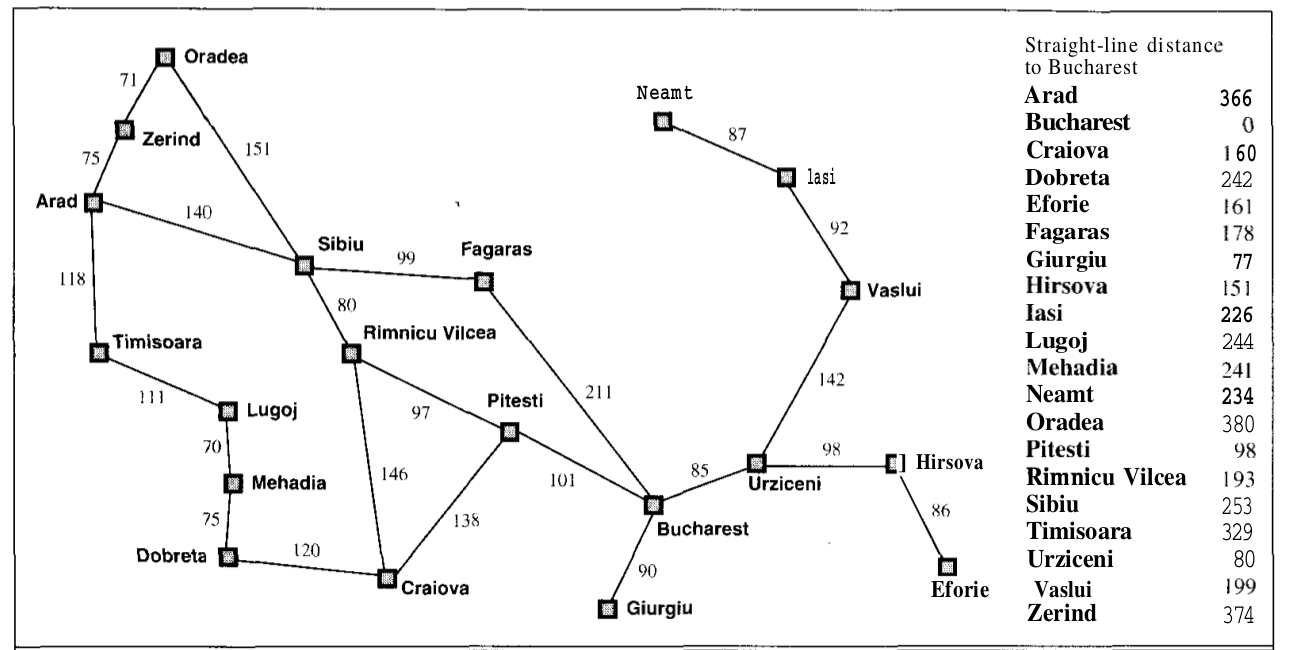
\includegraphics[width=.90\textwidth]{figuras/Aestrela-mapa1} 
\caption{Mapa da Romênia com os valores das distâncias entre as cidades, e a distância euclidiana até Bucareste.}
\label{fig-aestrela-algoritmo-mapa1}
\end{figure}

Um viajante deseja partir da cidade de Arad com destino a Bucareste buscando percorrer o menor caminho entre essas duas cidades. Para isso é utilizado o algoritmo A* que explora o grafos conforme descrito na figura \ref{fig-aestrela-algoritmo-mapa2}, tendo como heurística utilizada, a distância euclidiana entre todas as cidades e Bucareste (distâncias também contida na figura \ref{fig-aestrela-algoritmo-mapa1}).

\begin{figure}[H]
\centering
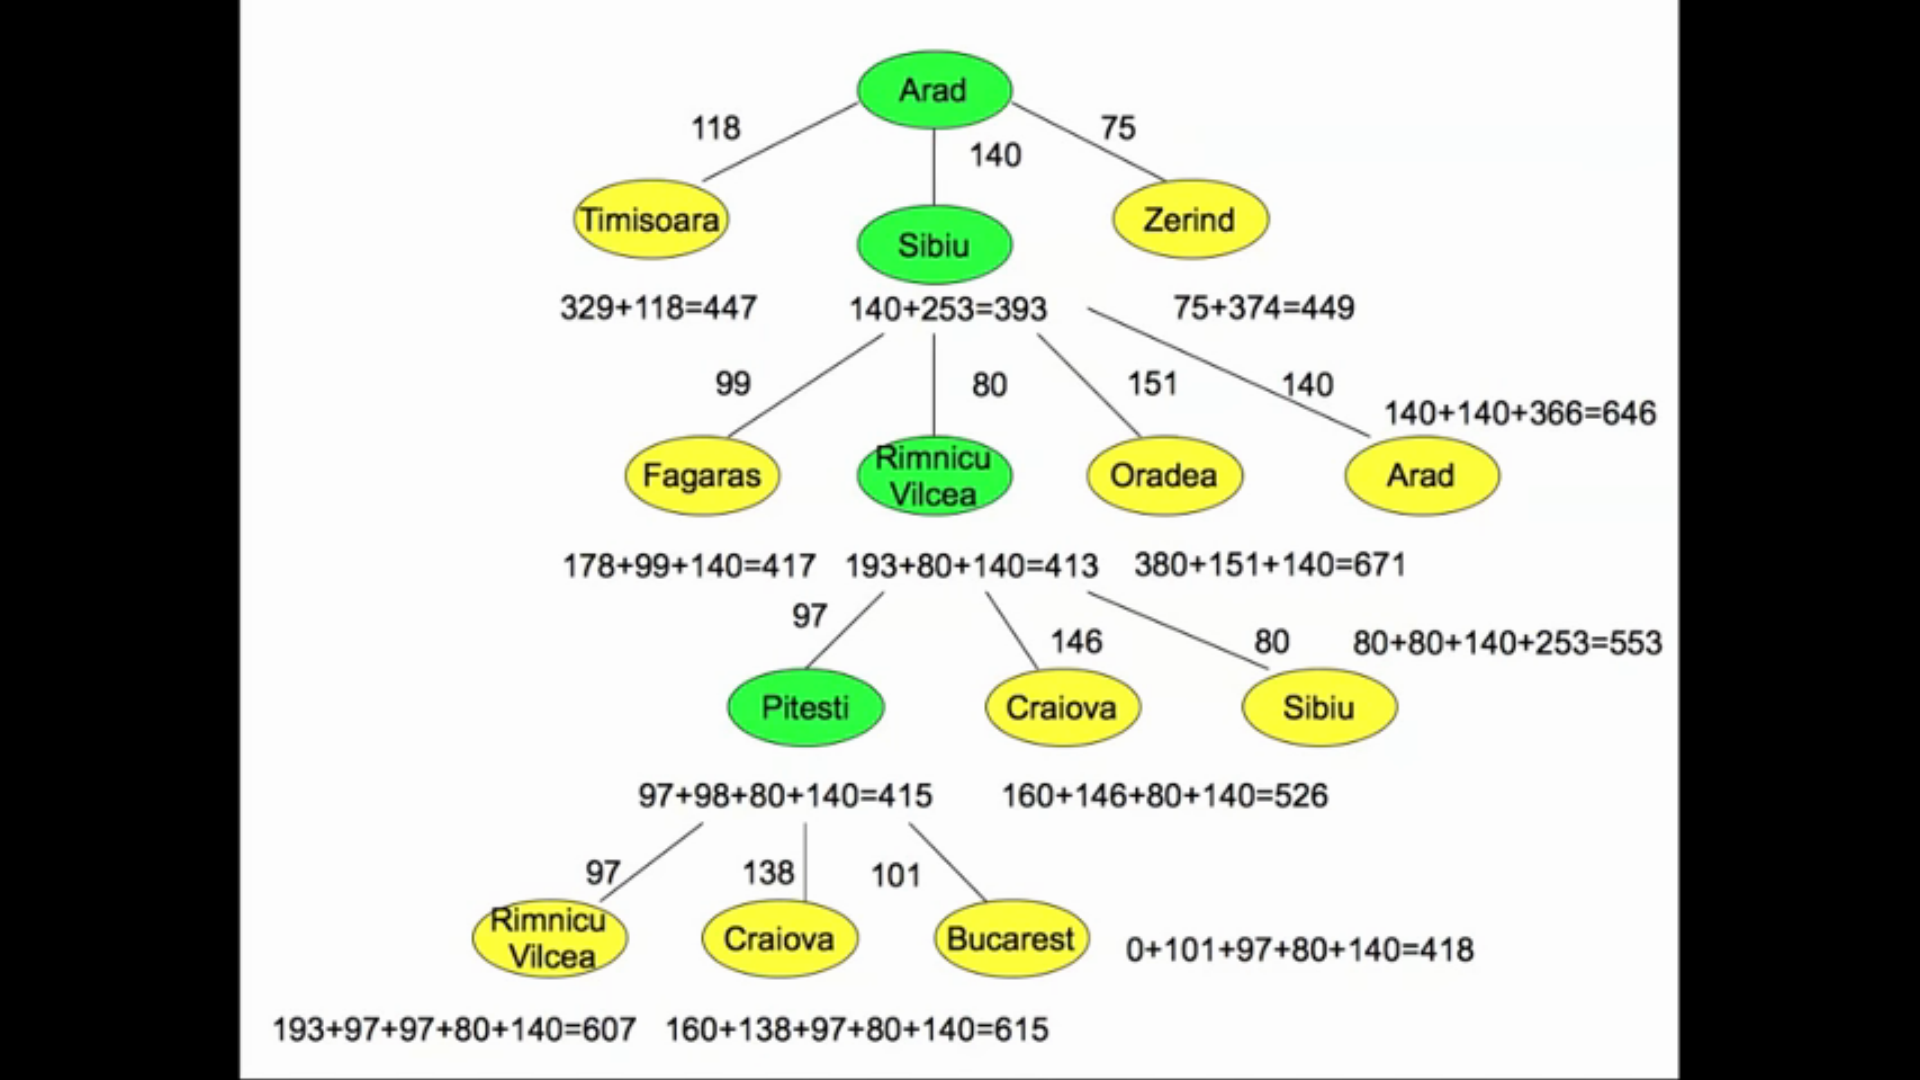
\includegraphics[width=.90\textwidth]{figuras/Aestrela-mapa2} 
\caption{Desenvolvimento do algoritmo A*.}
\label{fig-aestrela-algoritmo-mapa2}
\end{figure}




%\citeonline{russell1995modern,cormen2009introduction}.

%\begin{lstlisting}[ mathescape, label=lst-aestrela-codigo, caption=Algoritmo A*, float=htpb]
%Entrada: Grafo G, vértice inicial $v_{i}$, vértice destino $v_{f}$
%	para todo vértice $s \in V(G), s \neq vi$ faça
%		$g(s) = \infty$
%	fim para
%	$g(v_{i}) = 0$
%	para todo vértice $s \in V(G)$ faça
%		anterior($s$) = -1
%	fimpara
%	OPEN = {$v_{i}$}
%	enquanto $v_{f}$ não é expandido faça
%		s = desenfila(OPEN)
%		para cada sucessor $s'$ de $s$ faça
%			se $g(s') > g(s) + c(s,s')$ então
%				$g(s') = g(s) + c(s,s')$
%				anterior($s'$) = s
%				insira/atualize $s'$ em OPEN pelo valor de f
%			fim se
%		fim para
%	fim enquanto
%retorna anterior
%\end{lstlisting}



\subsection{Heurísticas admissíveis e não-admissíveis}
\label{sec-aestrela-algoritmo-heuristica}  
O fator heurístico h( u ) é uma estimativa da distância entre o vértice "u" e o vértice "goal". Ela é chamada de \textbf{admissível} quando o valor da estimativa garantidamente não superestima o valor da distância real entre "u" e "goal" \cite{russell1995modern}. Um exemplo clássico usado de heurística admissível é a distância euclidiana, já que a menor distância entre dois pontos é uma reta \cite{russell1995modern}.

O cálculo da distância euclidiana porém, nem sempre é a forma mais rápida em termos computacionais, já que geralmente ela é calculada em termos dos pontos geográficos do vértice e esse cálculo envolve exponenciação e radiação. É por isso que existe o uso de heurísticas \textbf{não-admissíveis}, que são estimativas que visam a usar cálculos mais simples, porém não há a garantia que essa distância superestime a distância real entre "u" e "goal", e com isso não há garantia que o melhor caminho seja encontrado.

Exemplos de heurísticas não-admissíveis:
\begin{itemize}
\item Distância Manhattan: h( u ) = $| x_{u} - x_{goal} | + | y_{u} - y_{goal}|$;
\item Atalho Diagonal: h( u ) = $\sqrt{2} * | y_{u} - y_{goal}| + ( | x_{u} - x_{goal} | - | y_{u} - y_{goal}| )$ [Se a distância $| x_{u} - x_{goal} | > | y_{u} - y_{goal}|$] || $\sqrt{2} * | x_{u} - x_{goal}| + ( | y_{u} - y_{goal}| - | x_{u} - x_{goal} | )$ [Se a distância $| x_{u} - x_{goal} | < | y_{u} - y_{goal}|$];
\end{itemize}

\section{Experimentos Computacionais}
\label{sec-aestrela-experimentos}

Para os experimentos computacionais serão utilizados as mesmas instâncias descritas em subseção \ref{sec-dijkstra-experimentos}. Serão comparados quatro versões de algoritmos: o algoritmo de Dijkstra descrito no capítulo \ref{sec-dijkstra}, o algoritmo de Dijkstra adaptado onde o algoritmo é parado assim que se é explorado o vértice objetivo, o algoritmo A* onde se utiliza a heurística admissível distância euclidiana e o algoritmo A* onde se utiliza a heurística não-admissível distância Manhattan, todas sumarizadas na tabela \ref{tbl-aestrela-instancias}.

\begin{table}[H]
\caption{Descrição das versões a serem testadas neste capítulo.}
\label{tbl-aestrela-instancias}
\centering
\begin{adjustbox}{max width=\textwidth}
\begin{tabular}{|c|c|}
\hline 
\textbf{Nome Instância} & \textbf{Descrição} \\ 
\hline 
Dijkstra & Versão de Dijsktra conforme descrito no capítulo \ref{sec-dijkstra} \\ 
\hline 
Dijkstra Adaptado & Versão de Dijkstra adaptado para parar quando o vértice destino é encontrado \\ 
\hline 
Algoritmo A* & Algoritmo A* utilizando a distância euclidiana \\ 
\hline 
Algoritmo A* Manhattan & Algoritmo A* utilizando a distância Manhattan \\ 
\hline 
\end{tabular} 
\end{adjustbox}
\end{table}

Será rodado dez vezes cada algoritmo para cada instância da subseção \ref{sec-dijkstra-experimentos} em que para cada rodada, será afixado o vértice origem como o sendo de valor de identificação "0" e terá como vértice destino um vértice escolhido aleatoriamente, sendo que não haverá repetição de vértices\footnote{Para o caso do algoritmo de Dijkstra especificado na primeira linha da tabela \ref{tbl-aestrela-instancias}, não será estabelecido um vértice destino já que o algoritmo calcula a melhor rota para todos os vértices do grafo.} (ou seja, supomos que o vértice de valor de identificação "180" tenha sido escolhido na primeira rodada. Esse vértice não será escolhido como destino nas demais 9 rodadas. Caso esse vértice seja "sorteado" na próxima iteração, um novo vértice será escolhido aleatoriamente). Nessas dez rodadas, será verificado o tempo médio de execução, o número médio de vértices abertos por cada versão e para o algoritmo A* com a heurística Manhattan, será verificado a qualidade da solução.

Para todas as versões, será utilizada a estrutura de dados Heap Binário (descrito na subseção \ref{sec-dijkstra-versoes-heap}) pois conforme mostrado no capítulo \ref{sec-dijkstra}, foi a estrutura que melhor se sobressaiu entre as outras em termos de tempo computacional.

\subsection{Resultados obtidos}
\label{sec-aestrela-instancias-resultados}

Os resultados dos testes computacionais descritos anteriormente podem ser vistos nas tabelas \ref{tbl-aestrela-resultados-tempo}, \ref{tbl-aestrela-resultados-qualidadesolucao} e \ref{tbl-aestrela-resultados-nva}.

\begin{table}[H]
\caption{Tempo médio obtido pelos métodos descritos na tabela \ref{tbl-aestrela-instancias} (tempo em milissegundos).}
\label{tbl-aestrela-resultados-tempo}
\centering
\begin{adjustbox}{max width=\textwidth}
\begin{tabular}{|c|c|c|c|c|}
\hline
\textbf{Nome Instância} & \textbf{Dijkstra} & \textbf{Dijkstra Adaptado} & \textbf{Algoritmo A*} & \textbf{Algoritmo A* Manhattan} \\ \hline
USA-road-d.NY.gr        & 236                           & 109                                    & 29                      & 14                                \\ \hline
USA-road-d.BAY.gr       & 321                           & 187                                    & 54                      & 23                                \\ \hline
USA-road-d.COL.gr       & 494                           & 229                                    & 117                     & 27                                \\ \hline
USA-road-d.FLA.gr       & 2858                          & 1026                                   & 886                     & 101                               \\ \hline
\end{tabular} 
\end{adjustbox}
\end{table}

\begin{table}[H]
\caption{Diferença média de solução obtida pelo A* Manhattan com relação a solução ótima.}
\label{tbl-aestrela-resultados-qualidadesolucao}
\centering
\begin{adjustbox}{max width=\textwidth}
\begin{tabular}{|c|c|}
\hline
\textbf{Nome Instância} & \textbf{Qualidade Solução} \\ \hline
USA-road-d.NY.gr        & 5\%                        \\ \hline
USA-road-d.BAY.gr       & 4\%                        \\ \hline
USA-road-d.COL.gr       & 3\%                        \\ \hline
USA-road-d.FLA.gr       & 3\%                        \\ \hline
\end{tabular} 
\end{adjustbox}
\end{table}

\begin{table}[H]
\caption{Número de Vértices Abertos (NVA) médio por cada método.}
\label{tbl-aestrela-resultados-nva}
\centering
\begin{adjustbox}{max width=\textwidth}
\begin{tabular}{|c|c|c|c|}
\hline
\textbf{Nome Instância} & \textbf{NVA Dijkstra Adptado} & \textbf{NVA A*} & \textbf{NVA A* Manhattan} \\ \hline
USA-road-d.NY.gr        & 140501                        & 31995           & 9079                      \\ \hline
USA-road-d.BAY.gr       & 225754                        & 53206           & 17044                     \\ \hline
USA-road-d.COL.gr       & 242674                        & 108343          & 21577                     \\ \hline
USA-road-d.FLA.gr       & 580010                        & 349201          & 79077                     \\ \hline
\end{tabular} 
\end{adjustbox}
\end{table}

\subsection{Análise dos resultados}
\label{sec-aestrela-resultados-analise}
Como apontado pelos testes realizados, o algoritmo A* teve um desempenho computacional melhor do que o algoritmo Dijkstra, inclusive sobre o Dijkstra Adaptado (descrito anteriormente). Podemos ver que esse resultado está diretamente ligado ao número de vértices abertos por cada algoritmo (tabela \ref{tbl-aestrela-resultados-nva}). Aqueles que abriram mais vértices, obtiveram um tempo computacional maior. Isso já esperado, já que o algoritmo teve que processar mais etapas até que sua condição de parada fosse encontrada.

Dos quatro métodos testados, o que obteve menor tempo computacional foi o algoritmo A* aplicando a heurística não-admissível Distância Manhattan. Isso se deve ao fato de o cálculo da distância (que é realizado em tempo de execução) ser mais simples do que o empregado pela distância euclidiana (que envolve radiação e exponenciação). Porém esse resultado possui um "preço a ser pago" que é, conforme descrito na subseção \ref{sec-aestrela-algoritmo-heuristica}, a não garantia do menor caminho entre os vértices pesquisados. Mas, conforme demonstra a tabela \ref{tbl-aestrela-resultados-qualidadesolucao}, a diferença média entre as soluções encontradas e suas respectivas soluções ótimas, giram em torno de 4\%, o que é pode ser considerado como um bom resultado.

\section{Conclusões}
\label{sec-aestrela-conclusao}




